\documentclass[../../main.tex]{subfiles}

\begin{document}

Il moto è il movimento dei corpi.
\subsection{Moto Rettilineo}
Il moto più semplice è il moto rettilineo, ovvero il moto lungo una retta. Inizialmente studiamo il moto di un corpo puntiforme.
Quando si parla di moto dobbiamo definire un'origine degli spazi e orientare la retta, in modo da determinare il verso positivo e
negativo.\\
Effettuando delle misurazioni si ottiene un diagramma orario e successivamente si può ottenere il grafico spazio-tempo.\\
\begin{figure}[h!]
    \centering
    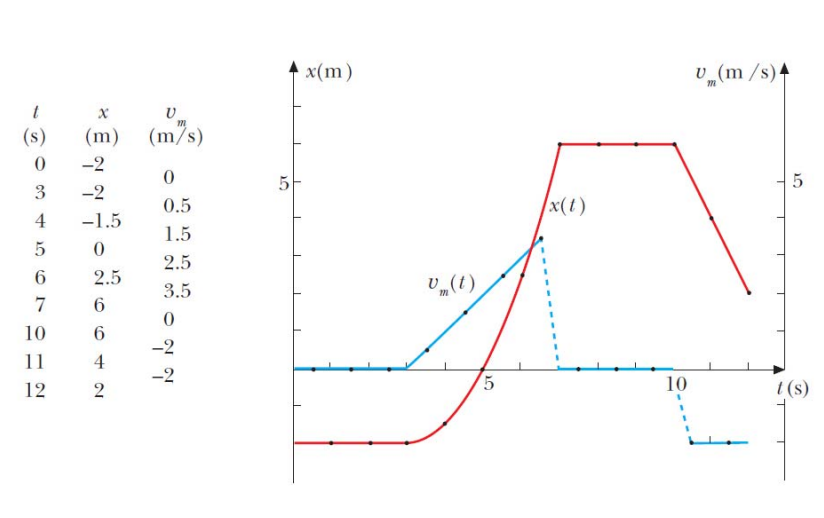
\includegraphics[width=0.6\textwidth]{Screenshot 2024-02-19 132549.png}
    \caption{Grafico spazio-tempo}
\end{figure}
\subsubsection{Velocità media}
Supponiamo che all'istante $t = t_1$ il punto si trovi nella posizione $x_1$ e all'istante $t = t_2$ nella posizione $x_2$.
La velocità media $v_m$ del punto è definita come il rapporto tra la variazione di spazio e l'intervallo di tempo in cui si è verificata la variazione di spazio.
\[
    \textbf{$\bar{v}_m$} = \frac{\Delta x}{\Delta t} = \frac{x_F - x_I}{t_F - t_I}
\]
La velocità media dà un'idea della rapidità con cui si muove il punto in un certo intervallo di tempo, ma non ci fornisce altre informazioni.
\subsubsection{Velocità istantanea}
Per individuare meglio le variazioni della funzione $x(t)$ si aumenta il numero delle misurazioni, riducendo l'intervallo di tempo.
Si divide l'intervallo di spazio $\Delta x$ in tanti intervalli di spazio $\Delta x_n$ e l'intervallo di tempo $\Delta t$ in tanti intervalli di tempo $\Delta t_n$. Le corrispondenti velocità medie sono $v_i = \frac{\Delta x_i}{\Delta t_i}$; questo processo può essere svolto per intervalli di tempo sempre più piccoli, fino a giungere a un intervallo di tempo infinitesimo $\Delta t \to 0$.
\[
    \textbf{v} = \lim_{\Delta t \to 0} \frac{\Delta x}{\Delta t} = \frac{dx}{dt}
\]
La velocità istantanea è una variazione piccolissima variazione di spazio in un piccolissimo intervallo di tempo.\\
Possiamo risolvere il problema inverso, cioè ricavare la funzione $x(t)$ se conosciamo la dipendenza dal tempo della velocità istantanea $v(t)$. Se il punto si trova nella posizione $x$ al tempo $t$ e nella posizione $x + dx$ al tempo $t + dt$, lo spostamento infinitesimo $dx$ è uguale al prodotto della velocità istantanea per l'intervallo di tempo infinitesimo $dt$:
\[
    dx = v(t) \cdot dt \implies \int_{x_0}^{x} dx = \int_{t_0}^{t} v(t) \cdot dt \implies x(t) = x_0 \int_{t_0}^{t} v(t) \cdot dt
\]
\subsubsection{Due punti in moto sullo stesso asse}
Due punti materiali si trovano nell’istante iniziale $t = 0$ sullo stesso asse $x$, rispettivamente nella posizione $x_1$ con
velocità $v_1$ e nella posizione $x_2 > x_1$ con velocità $v_2$. Il moto dei punti è uniforme. Discutere quali sono le situazioni in
cui i punti ad un certo istante si urtano e determinare dove e quando si urtano.\\ Moto rettilineo uniforme $\iff$ velocità costante.\\
\[
    v = \frac{dx}{dt} \implies dx = v \cdot dt \implies \int_{0}^{t_0} dx = \int_{0}^{t_0} v(t) \cdot dt
\]
\[
    x(t_0) - x(0) = \int_{0}^{t_0} v(t) \cdot dt \implies x(t_0) - x(0) = \int_{0}^{t_0} v \cdot dt \implies x(t_0) - x(0) = v_0(t_0 - 0) \implies x(t_0) = v_0 \cdot t_0
\]
\[
    x_1(t) = v_1 \cdot t \quad x_2(t) = v_2 \cdot t + x_2(0)
\]
\begin{figure}[h!]
    \centering
    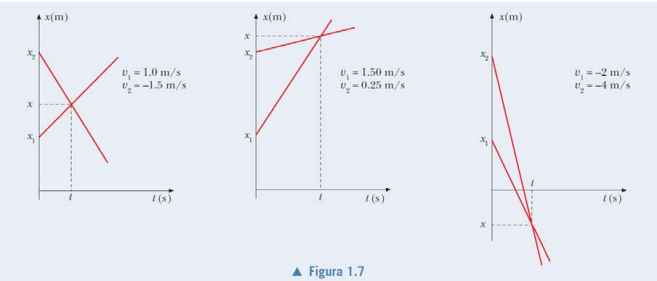
\includegraphics[width=0.8\textwidth]{9a2591ca-93e4-42c3-a861-5f067fd67bdb.png}
    \caption{Esempi di grafici di due punti in moto sullo stesso asse}
\end{figure}

\subsection{Accelerazione nel moto rettilineo}
Si definisce accelerazione e si indica con $\bar a$ il rapporto tra la velocità in un certo istante e l'intervallo di tempo in cui si è verificata la variazione di velocità.
\[
    a_m = \frac{\Delta v}{\Delta t} = \frac{v_2 - v_1}{t_2 - t_1}
\]
\[
    a_i = \lim_{\Delta t \to 0} \frac{\Delta v}{\Delta t} = \frac{dv}{dt} \implies v = \frac{dx}{dt} \implies a = \frac{d^2x}{dt^2}
\]
Anche quando la velocità diminuisce si ha un'accelerazione, ma negativa.\\
Se conosco l'accelerazione posso calcolare la velocità.
\[
    \dfrac{dv}{dt} = a \implies \int_{v_0}^{v_1} dv = \int_{0}^{t_1} a \cdot dt \implies v_1 - v_0 = \int_{t_0}^{t_1} a(t) \cdot dt
\]
\[
    v(t) = v(t_0) + \int_{t_0}^{t} a(t) \cdot dt
\]
\subsection{Moto rettilineo uniformemente accelerato}
Moto rettilineo uniformemente accelerato $\iff$ accelerazione costante.\\
Le equazioni del \textbf{moto rettilineo uniformemente accelerato} sono:
\[
    \begin{cases}
        v(t) = v_0 + a \cdot t \\
        x(t) = x_0 + v_0t + \dfrac{1}{2}at^2
    \end{cases}
\]
\[
    dv = a dt \implies \int_{v_0}^v dv = \int_{0}^t a dt \implies v - v_0 = a \int_{0}^t dt = a \cdot t \implies v = v_0 + a \cdot t
\]
\[
    v = \dfrac{dx}{dt} \implies dx = v \cdot dt \implies dx = [v_0 + a(t - t_0)]dt \implies \int_{x_0}^x dx = \int_{t_0}^t v_0 dt + \int_{t_0}^t a(t - t_0) dt
\]
\[
    x - x_0 = v_0(t - t_0) + \dfrac{1}{2} a(t - t_0)^2
\]
\subsubsection{Esercizio}
Un’automobile è in grado di passare dalla quiete alla velocità di $100 \frac{km}{h}$ in $t$ secondi, muovendosi con moto
uniformemente accelerato. Esprimere il valore dell’accelerazione e calcolarlo per $t = t1 = 5 s$ e per $t = t2 = 8 s$. Quanto
vale lo spazio percorso nei due casi? E la velocità media?\\
\vspace*{0.1cm} \\
\textbf{Risoluzione:} \\
\begin{math}
    v = at \implies a = \dfrac{v_f}{t} \\
    \vspace*{0.1cm} \\
    v_f = 100 \dfrac{km}{h} = 27.78 \dfrac{m}{s} \\
    \vspace*{0.1cm} \\
    a = \dfrac{27.78 \dfrac{m}{s}}{5s} = 5.56 \dfrac{m}{s^2} \\
    \vspace*{0.1cm} \\
    a_2 = \dfrac{27.78 \dfrac{m}{s}}{8s} = 3.47 \dfrac{m}{s^2} \\
    \vspace*{0.1cm} \\
    x = x_0 + v_0t + \dfrac{1}{2}at^2 \\
    \vspace*{0.1cm} \\
    \implies x_1 = 0 + 0 + \dfrac{1}{2} \cdot 5.56 \dfrac{m}{s^2} \cdot 5^2s^2 = 69.5m \\
    \vspace*{0.1cm} \\
    \implies x_2 = 0 + 0 + \dfrac{1}{2} \cdot 3.47 \dfrac{m}{s^2} \cdot 8^2s^2 = 111m \\
    \vspace*{0.1cm} \\
    \bar{v}_{m_1} = \dfrac{69.5m}{5s} = 13.9 \dfrac{m}{s} \\
    \vspace*{0.1cm} \\
    \bar{v}_{m_2} = \dfrac{111m}{8s} = 13.9 \dfrac{m}{s} \\
\end{math}

\subsubsection{Esercizio accelerazione negativa}
Un punto materiale parte dall’origine con velocità iniziale $v_0$ positiva ed è sottoposto ad un’accelerazione negativa –
a costante. Calcolare la massima distanza dall’origine raggiunta dal punto lungo il semiasse positivo, l’istante $t_1$ in
cui si ferma, l’istante $t_2$ in cui ripassa per l’origine e la velocità che ha per $t = t_2$.\\
\vspace*{0.5pt} \\
\begin{math}
    v = v_0 + at \implies v_0 + at, \ a < 0, \ v_0 > 0 \\
    \vspace*{0.1cm} \\
    v_0 + at = 0 \implies t_1 = \dfrac{-v_0}{a} \\
    \vspace*{0.1cm} \\
    x = x_0 + v_0t + \dfrac{1}{2}at^2 \implies x_1 = v_0 \cdot t_1 + \dfrac{1}{2}at_1^2 =  \dfrac{-v_0^2}{a} + \dfrac{1}{2}a \cdot \dfrac{v_0^2}{a^2} = \dfrac{-v_0^2}{2a} \\
    \vspace*{0.1cm} \\
    \textit{Ora calcoliamo quando il punto ripassa per l'origine} \ \
    v_0 + \frac{1}{2} at^2 = 0 \begin{cases}
        t = 0 \\
        t_2 = \dfrac{2v_0}{-a}
    \end{cases}\\
    \vspace*{0.1cm} \\
    \textit{Velocità in } t_2 \ \ v_2 = v_0 + at_2 = v_0 - 2v_0 = -v_0 \\
\end{math}

\section{Valori Medi}
\subsection{Valore medio di una funzione}
\[
    <f(t)> = \dfrac{\int_{0}^{T} f(t) dt}{T}
\]
Nel caso della funzione $\sin$, la media su un periodo è nulla: \\
\[
    <\sin(t)> = \dfrac{1}{2\pi} \int_{0}^{2\pi} \sin(\theta) d\theta = \dfrac{1}{2\pi} \left[ -\cos(\theta) \right]_{0}^{2\pi} = 0
\]
Lo stesso si ottiene per il coseno, ed è evidente, basta osservare il grafico; in un semiperiodo la funzione è positiva, nell'altro è negativa e la loro somma è nulla.\\
E' diversa la situazione per la funzione $\sin^2$ e $\cos^2$, funzioni che hanno come periodo $\pi$, che essendo
sempre positive non possono aver valore medio nullo. Osserviamo che:
\[
    \int_0^\pi (\sin^2(\theta) + \cos^2(\theta)) d\theta = \int_0^\pi 1 d\theta = \pi
\]
pertanto
\[
    \int_0^\pi \int^2(\theta) d\theta = \int_0^\pi \cos^2(\theta) d\theta = \dfrac{\pi}{2}
\]

\subsubsection{Esercizio 1.4 (compito)}

\section{Moto verticale di un corpo}
Un corpo in caduta libera è un corpo che cade sotto l'azione della forza di gravità.\\
\[
    g = 9.81 \dfrac{m}{s^2}
\]
\[
    \begin{cases}
        v = v_0 - g \cdot t \\
        x = x_0 + v_0t - \dfrac{1}{2}gt^2
    \end{cases}
\]
\begin{figure}[!h]
    \centering
    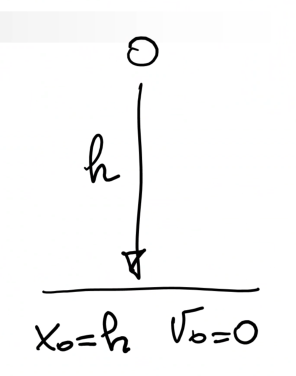
\includegraphics[width=0.3\textwidth]{Screenshot 2024-02-20 093133.png}
    \caption{Esercizio 1.6}
\end{figure}\[
    0 = h +v_0\bar{t}-\frac{1}{2}g\bar{t}^2 \implies \bar{t} = \sqrt{\dfrac{2h}{g}}
\]
\subsubsection{Esercizio 1.6}
Un punto materiale viene lasciato cadere all’istante $t = 0$ con velocità iniziale nulla. Un secondo punto materiale
viene lanciato verso il basso all’istante $t = t_0 > 0$, con velocità iniziale $v_0$: riuscirà a raggiungere il primo punto?
\begin{figure}[!h]
    \centering
    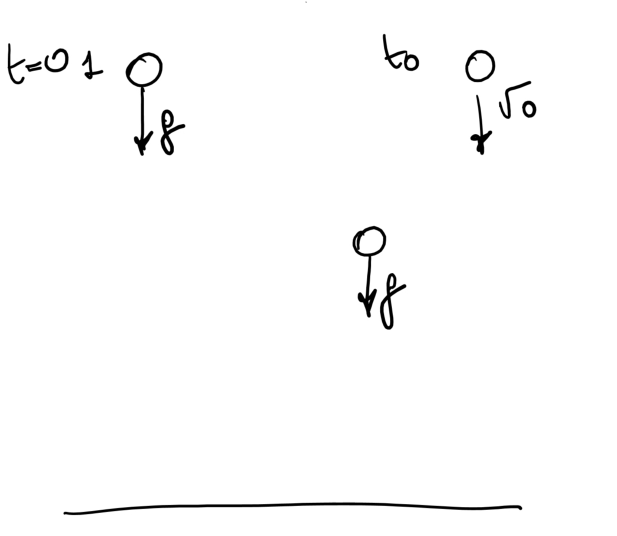
\includegraphics[width=0.5\textwidth]{Disegno1-6.png}
    \caption{Esercizio 1.6}
\end{figure}
\vspace*{0.1cm} \\
\begin{math}
    x_1(t) = \dfrac{1}{2}gt^2 \textit{ perchè abbiamo considerato il punto di partenza $h$ come l'origine} \\
    x_2(t) = v_0(t - t_0) + \dfrac{1}{2}g(t-t_0)^2 \textit{ perchè il secondo corpo viene lasciato cadere in un secondo istante $t_0$} \\
    \textit{si incontrano a } \bar{t} = x_1(\bar{t}) = x_2(\bar{t}) \implies \dfrac{1}{2}g\bar{t}^2 = v_0(\bar{t} - t_0) + \dfrac{1}{2}g(\bar{t}-t_0)^2 \\
    \bar{t} = \dfrac{t_0}{2} \left(1+\dfrac{v_0}{v_0-gt_0}\right)
\end{math}

\section{Moto Armonico}
\subsection{Moto armonico semplice}
Un corpo si muove di moto armonico se la sua posizione in funzione del tempo è descritta da:
\[
    x(t) = A \cdot \sin(2\pi t)
\]
\[
    x(t) = A \cdot \sin(\omega t + \phi)
\]
Periodo della funzione: quale è il valore di $t : x(t) = x(t + T)$?
\[
    T = \dfrac{2\pi}{\omega} \textit{ è il periodo}
\]
\[
    \omega = \dfrac{2\pi}{T} \textit{ è la pulsazione angolare}
\]
\[
    x(t) = A \cdot \sin(\omega t + \phi) = x(t+T) = A \cdot \sin(\omega t+\dfrac{\omega2\pi}{\omega}+\phi)
\]
La frequenza del moto misura il numero di cicli che si compiono in un secondo:
\[
    f, \ \nu = \mathbf{\dfrac{1}{T}} \textit{ è l'inverso del periodo e si misura in } s^{-1} \textit{ o } Hz
\]
\[
    v = \dfrac{dx}{dt} = \mathbf{A \cdot \omega \cdot \cos(\omega t + \phi)}
\]
\[
    a = \dfrac{dv}{dt} = \mathbf{-A \cdot \omega^2 \cdot \sin(\omega t + \phi)}
\]
oppure
\[
    a = -\omega^2 \cdot x(t)
\]
\[
    \int_{x_0}^{x} -\omega^2xdx = \dfrac{1}{2} v^2 - \dfrac{1}{2}v_0^2 \implies \ -\omega^2[\frac{1}{2}x^2]_{x_0}^{x}
\]
\[
    v^2 = v_0^2 - 2\omega^2(x-x_0)
\]
\begin{figure}[h!]
    \centering
    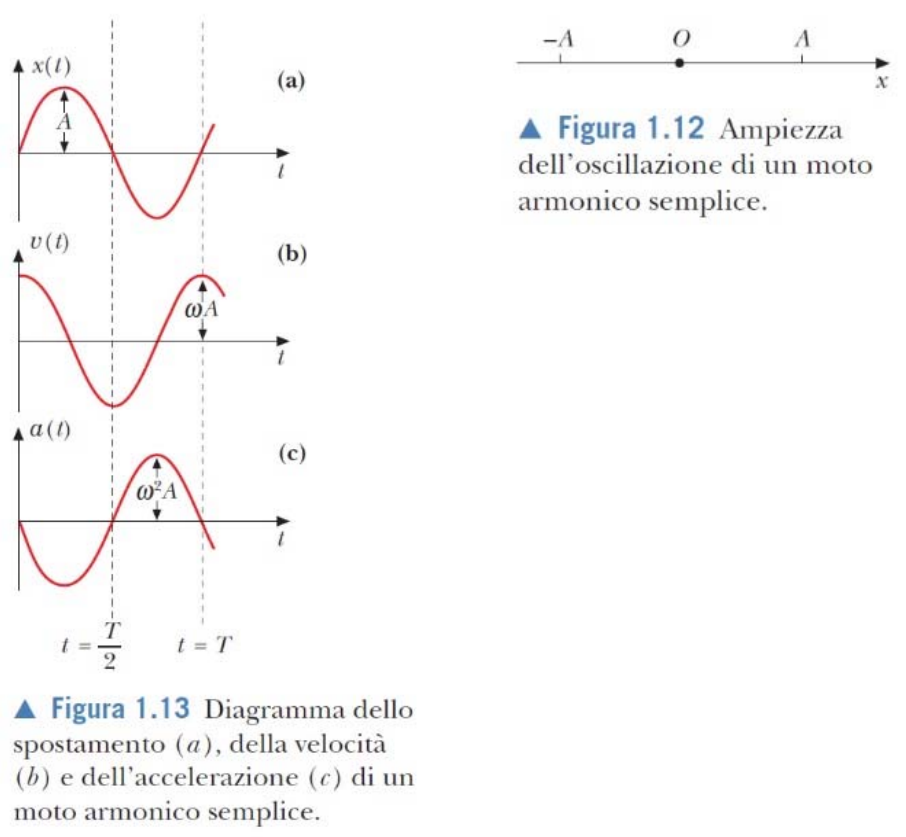
\includegraphics[width=0.5\textwidth]{armonico.png}
    \caption{Moto armonico}
\end{figure}
\begin{math}
    x(t) = A\sin(\omega t + \phi) \ \ \ \ t = 0 \ \ \ \ x(0) = A\sin(\phi) \\
    v(t) = A\omega\cos(\omega t + \phi) \ \ \ \ t = 0 \ \ \ \ v(0) = A\omega\cos(\phi)
\end{math}
\\In base alla velocità iniziale a alla posizione iniziale possiamo determinare $\phi$:
\begin{math}
    x(0) = x_0 = A \\
    v(0) = 0
    \implies \begin{cases}
        A\sin(\phi) = A \\
        A\omega\cos(\phi) = 0
    \end{cases}
    \implies \phi = \frac{\pi}{2}
\end{math}
Omega invece è legato a come è impostato il sistema.

\section{Velocità e accelerazione in funzione della posizione}
\[
    a = \dfrac{dv}{dt} = \dfrac{dv[x(t)]}{dt} = \dfrac{dv}{dx} \cdot \textcolor{red}{\dfrac{dx}{dt}}
\]
\[
    \implies \textcolor{red}{\int_{x_0}^x adx = \int_{v_0}^v vdv \implies \int_{x_0}^x adx = \frac{1}{2}v^2 - \frac{1}{2}v_0^2}
\]

\subsubsection{Un particolare moto vario esempio 1.7}
Un punto materiale risente, lungo l’asse x positivo, della seguente accelerazione: $a = 0 per 0 \leq x \leq x0$, a = –
k/x 2 per x > x0. Il punto viene lanciato dall’origine lungo il verso positivo dell’asse con velocità iniziale v0. Calcolare
in quale posizione il punto si ferma e discutere il risultato.
\[
    \int_{x_0}^{x} adc = \frac{1}{2}v^2 - \frac{1}{2}v_0^2 \ \ \ \ a =\textit{ costante} \ \ \ a(x-x_0) = \frac{1}{2}v^2 - \frac{1}{2}v_0^2
\]
\[
    v = v_0 - gt
\]
\[
    x = h - \frac{1}{2}gt^2
\]
\[
    g(x-h) = \frac{1}{2}v^2 - \frac{1}{2}v_0^2
\]
\[
    v(x) = \sqrt{2g(x-h) + v_0^2}
\]




\end{document}
